\documentclass[a4paper,12pt]{article}

\author{}
\date{}
\title{Filtration of Ideal Gas and Pentane \(\left( C_5 H_{12} \right) \)}

\usepackage[margin=0.9in]{geometry}
\usepackage{graphicx}
\usepackage{float}
\usepackage{textcomp}
\usepackage{amsmath, amssymb}
\usepackage{siunitx}
\usepackage{subcaption}
\usepackage{multirow}
\usepackage{bm}
\usepackage{ulem}
\usepackage{xcolor}

\definecolor{grey}{HTML}{737373}
\definecolor{red}{HTML}{d9343f}
\definecolor{green}{HTML}{2e8a07}

\begin{document}
\maketitle
\section{The Physics}
We simulate 2d flow of ideal gas and \(C_5H_{12}\) through a
porous medium with the help of Darcy's law:
\begin{equation}
    \bm{v}_i = -\frac{1}{\mu_i} \hat K \cdot f_\alpha (s)
    \cdot \nabla P
\end{equation}
where \(\hat K\), the specific permeability.
It depends only on the geometry of the medium.
We assume isotropy of space, so K is a scalar.
\(\mu\) is the dynamic viscosity.

\(i\) - component.

\(\alpha\) - phase. (If we had multiple phases, then
it would be \(f_\alpha\))

As an approximation, \(f_\alpha (s) = s^2\) for the first 
component, and \(f_\alpha (s) = (1 - s)^2\) for the second.

The continuity equation for each component becomes:
\begin{equation}
    \varphi \frac{\partial \rho_i}{\partial t}
    + div (\rho_i \bm{v}_i) = 0
\end{equation}
where \(\rho_i = \frac{m_i}{V}\).

We use the Tait equation to relate liquid density to pressure:
\begin{equation}
    \frac{\rho - \rho_0}{\rho} = C \log_{10}
    \frac{B + P}{B + P_0}
\end{equation}
where \(C = 0.2105\),
\(\rho_0 = \frac{1}{67.28 \frac{m^3}{mol}}\),
\(P_0 = 0.1 MPa\), \(B = 35MPa\),
in the case of \(C_5H_{12}\).

Ideal gas equation of state:
\begin{equation}
    P = \frac{RT}{M}\rho
\end{equation}

\section{Boundary and Initial Conditions}

On the first iteration, we set an initial
pressure and molar composition.
Then, we derive the velocities from the 
pressure gradient using Darcy's law and the
saturation from the densities
and molar composition.

{\color{red}All our BC are 2-nd order (thanks to ghost
    cells), except for the BC on velocity on the inlet
and outlet, which end up being 1-st order.}

\begin{figure}[H]
    \centering
    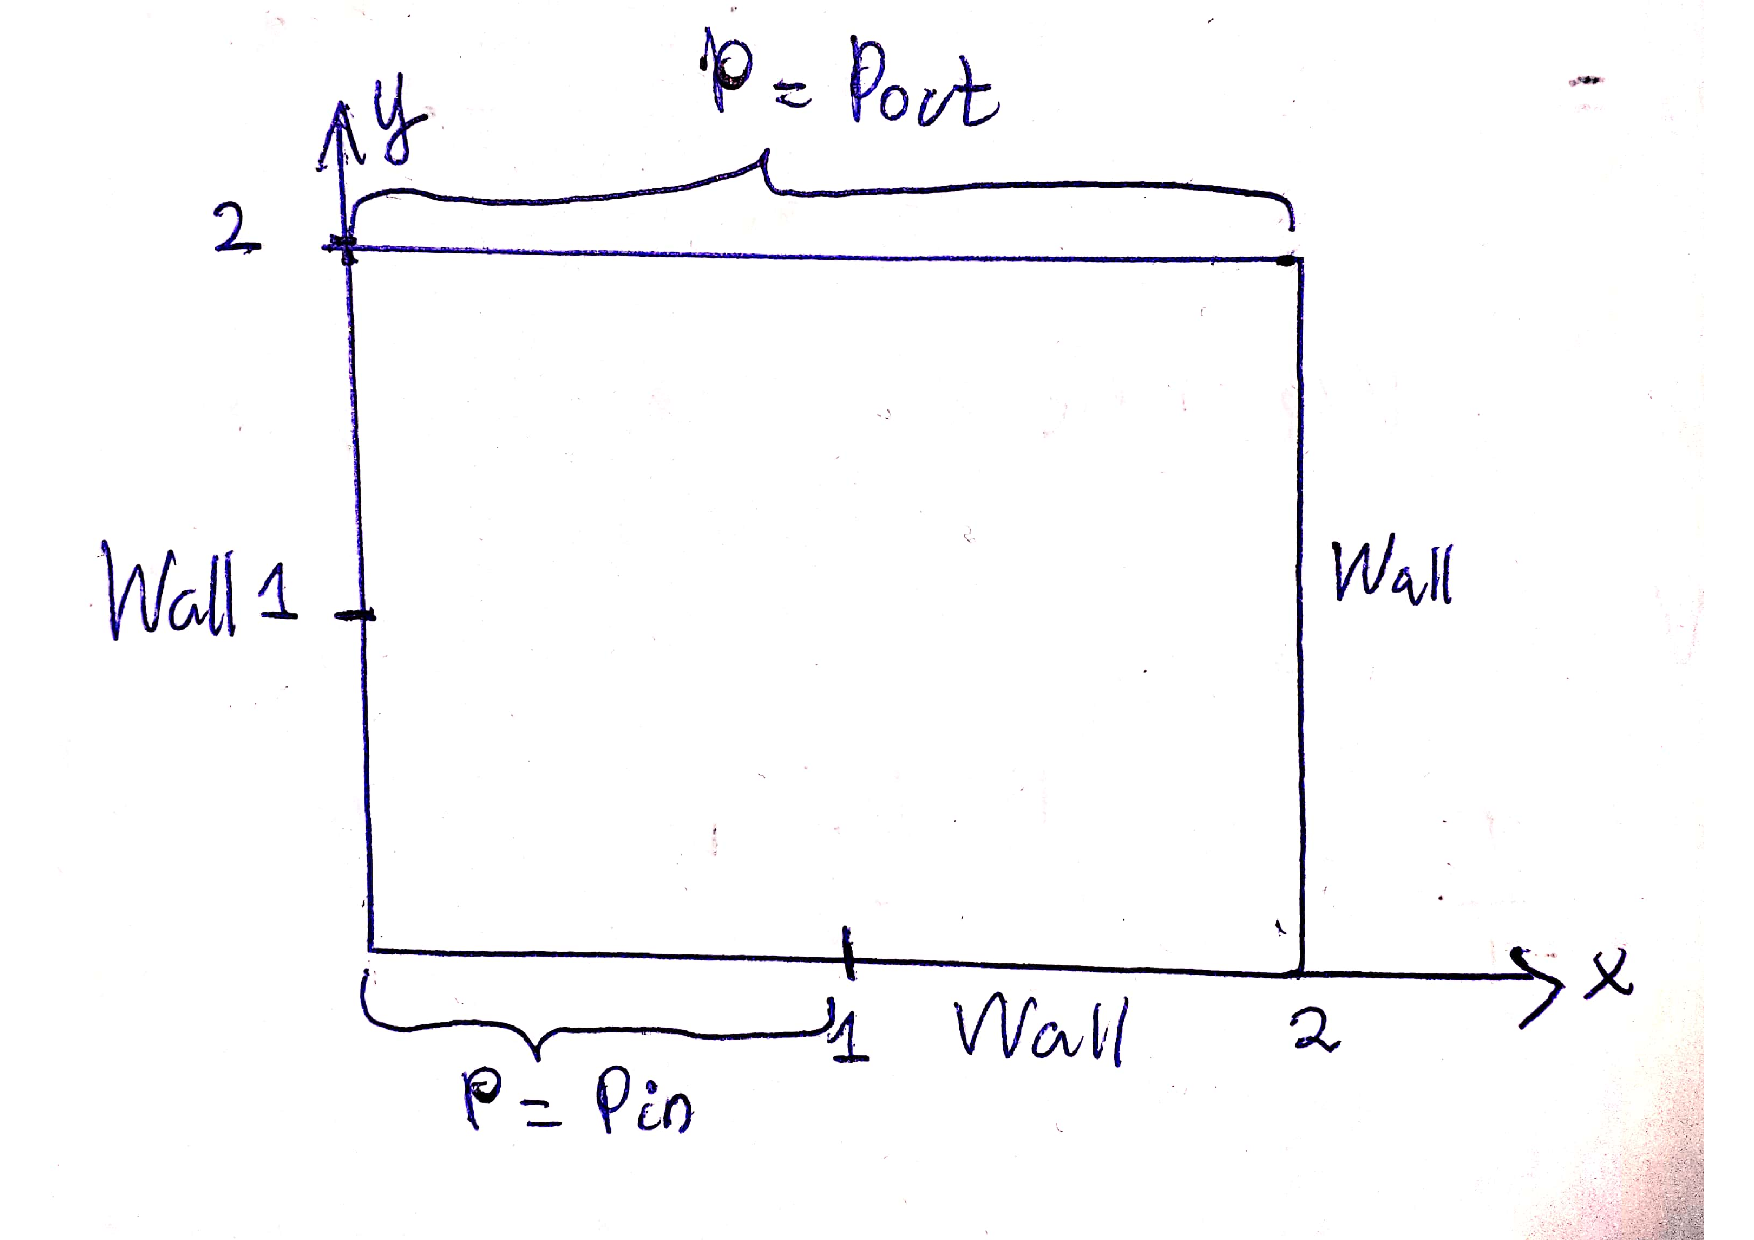
\includegraphics[width=0.5\textwidth]{img/diagram.pdf}
    \caption{Boundary Conditions}
    \label{fig:img-diagram-pdf}
\end{figure}

\subsection{Pressure}

\textbf{BC:}

\[
\begin{cases}
    P = P_{in} &\text{at } y = 0
    \text{ and } x \in [0, 1] \\
    P = P_{out} &\text{at } y = 2 \\
    \frac{\partial P}{\partial x} = 0 &\text{at }
    x = 0, 2 \\
    \frac{\partial P}{\partial y} = 0 &\text{at }
    y = 0 \text{ and } x \in [1, 2]
\end{cases}
\] 

\textbf{IC:}

\[
\begin{cases}
    P = P_{out} &\text{at outlet} \\
    P = P_{in}  &\text{at inlet} \\
    P = P_0     &\text{everywhere else}
\end{cases}
\] 

\subsection{Velocities}

\textbf{IC:} Darcy 1-st order.

\textbf{BC:}

\[
\begin{cases}
    u = 0 &\text{at } x = 0, 2 \\
    v = 0 &\text{at } y = 0 \text{ and } x \in [1, 2] \\
    {\color{red}\text{Darcy (1-st Order)}}
          &\text{at } y = 2 \\
    {\color{red}\text{Darcy (1-st Order)}}
          &\text{at } y = 0
    \text{ and } x \in [0, 1]\\
\end{cases}
\] 

\subsection{Density}

We derive the densities from the equations of state.

\subsection{Saturation}
    Boundary condition on the inlet as the molar
    composition:
    \[
        \psi = \frac{\nu_1}{\nu_2} = \frac{m_1}{M_1}
        \cdot \frac{M_2}{m_2},
    \] 
    where \(M_1\) and \(M_2\) represent the molar mass 
    of each component.

    We can derive the densities from the equations of state,
    then we can find the saturation.

    \[
    \rho_1 = \frac{m_1}{sV}, \qquad
    \rho_2 = \frac{m_2}{(1 - s)V}
    \] 

    \[
    \frac{\rho_1}{\rho_2} = \frac{m_1}{m_2}
    \frac{1 - s}{s}
    = \psi \frac{M_2}{M_1}\frac{1 - s}{s}
    \] 

    \[
        s = \left( 
        \frac{\rho_1 M_1}{\rho_2 M_2 \psi} + 1 \right)^{-1}
    \] 

    {\color{red}What about everywhere else???}

\section{Discretization Scheme}

We use the finite difference method (FDM).

\subsection{Continuity Equation}

Second order in space. First order in time.

\[
\frac{\partial \rho}{\partial t}
+ \frac{\partial \rho}{\partial x} u
+ \frac{\partial \rho}{\partial y} v
+ \frac{\partial u}{\partial x} \rho
+ \frac{\partial v}{\partial y} \rho = 0
\] 

\[
\varphi \frac{\rho^{n + 1}_{i, j} - \rho^n_{i, j}}{\Delta t}
+ \frac{\rho_{i+1, j}^n - \rho_{i-1,j}^n}{2\Delta x} u_{i,j}
+ \frac{\rho_{i, j+1}^n - \rho_{i,j-1}^n}{2\Delta y} v_{i,j}
+ \frac{u_{i+1, j} - u_{i-1,j}^n}{2\Delta x} \rho_{i,j}^n
+ \frac{v_{i, j+1}^n - v_{i,j-1}^n}{2\Delta y} \rho_{ij}^n = 0
\] 

\subsection{Darcy's Law}

Second order in space.

\[
    u_{i,j}^n = -\frac{K}{\mu} f_\alpha (s_{i, j}^n)
    \frac{P_{i + 1, j}^n - P_{i - 1, j}^n}{2\Delta x} \\
\] 

\[
    v_{i,j}^n = -\frac{K}{\mu} f_\alpha(s_{i, j}^n)
    \frac{P_{i, j + 1}^n - P_{i, j - 1}^n}{2\Delta y}
\] 

\section{Algorithm}

Euler method for discretization with respect to time.
(TODO: upgrade to predictor-corrector).

Second order scheme in space, with the use of ghost cells. 

\begin{enumerate}
    \item Calculate densities for each component using EOS.
    \item Find the pressure and saturation with the
        help of binary search.
    \item Use Darcy's law to calculate velocities.
\end{enumerate}

\section{Units and Parameters}

\begin{table}[H]
    \centering
    \caption{Parameters for our simulation.}
    \label{tab:label}
    \begin{tabular}{| c | c |}
        \hline
        Temperature & 298 \(K\) \\
        \hline
        \(P_{in}\) & \(10^6 Pa\) \\
        \hline
        \(P_{out}\) & \(10^5 Pa\) \\
        \hline
        Porosity, \(\varphi\) & 0.7 \\
        \hline
        Specific Permeability, \(K\) & \(10^{-12}\) \\
        \hline
        Dynamic Viscosity of Ideal Gas, \(\mu_1\) &
        \(1.8 \cdot 10^{-5}\) \(Pa \cdot s\) \\
        \hline
        Dynamic Viscosity of Pentane, \(\mu_2\) &
        \(2,14 \cdot 10^{-4}\) \( Pa \cdot s\) \\
        \hline
        Molar Mass of Ideal Gas, \(M_1\) & 
        \(0.028\) \(\frac{kg}{mol}\) \\
        \hline
        Molar Mass of Pentane, \(M_2\) & 
        \(0.07215\) \(\frac{kg}{mol}\) \\
        \hline
        Molar Composition at Inlet, \(\psi\) &
        \(0.3\) \\
        \hline
    \end{tabular}
\end{table}

\section{TODO}

\begin{enumerate}
    \item \sout{Fix: \(\mu\) is different for each component.}

    % \item Add boundary conditions on \(s_{n + 1} = s_n\)
    %     in the borders.

    \item \sout{Calculate the velocities in the first 
        iteration with a first order scheme. 
    Then, everything is calculated as normal.}

    \item \sout{The boundary condition \(\frac{dv}{dn} = 0\) 
            is usually used when solving the Navier-Stokes
        equation. In the case of filtration with Darcy's
        equation, we can either set the velocities
        explicitly or derive them from the pressure
        gradient on the boundaries and from the Darcy's
    equation on the inside.}

    \item \sout{Create boundary condition on the inlet 
            as the molar
        composition:}
        \[
            \psi = \frac{\nu_1}{\nu_2} = \frac{m_1}{M_1}
            \cdot \frac{M_2}{m_2},
        \] 
        \sout{where \(M_1\) and \(M_2\) represent 
            the molar mass of each component.

        This way, we are essentially giving a boundary
        condition on the saturation, since we can derive
    the densities from the equations of state.}

    \item Change order of indexing: column major storage
        in memory.

    \item Use naming conventions consistent with Julia base.

Functions are lowercase (maximum, convert) and, when readable, 
with multiple words squashed together.
When necessary, use underscores as word separators.

    \item Upgrade to predictor-corrector
\end{enumerate}
\end{document}
